%\documentclass[aspectratio=169, handout]{beamer}
\documentclass[aspectratio=169]{beamer}


\usefonttheme{professionalfonts}
\usetheme{boxes}
\mode<presentation>
%{
%  \usecolortheme{whale}%whale
%  % or ...
%  \setbeamercovered{transparent}
%  \definecolor{BerkeleyBlue}{RGB}{0,50,98}
%  \definecolor{UtahRed}{RGB}{204,0,0}
%  \definecolor{DarkGreen}{RGB}{0,128,0}
%%\setbeamercolor{title}{fg=BerkeleyBlue}
%%\setbeamercolor{frametitle}{fg=BerkeleyBlue}
%\setbeamercolor{structure}{fg=BerkeleyBlue}
%}

\usepackage{tikz}
\usetikzlibrary{tikzmark,fit,shapes.geometric}


\newcommand{\transp}{^{\rm{T}}}

\usepackage{cases}
\usepackage[english]{babel}
% or whatever
\usepackage{xcolor}
\usepackage{colortbl}
\usepackage[latin1]{inputenc}
\usepackage[super]{nth}
% or whatever
%\setbeamertemplate{footline}[page number]
\setbeamertemplate{footline}
        {
      \leavevmode%
      \hbox{%
      \begin{beamercolorbox}[wd=.333333\paperwidth,ht=2.25ex,dp=1ex,center]{author in head/foot}%
        \usebeamerfont{author in head/foot}\insertshortauthor%~~(\insertshortinstitute)
      \end{beamercolorbox}%
      \begin{beamercolorbox}[wd=.333333\paperwidth,ht=2.25ex,dp=1ex,center]{title in head/foot}%
        \usebeamerfont{title in head/foot}\insertshorttitle
      \end{beamercolorbox}%
      \begin{beamercolorbox}[wd=.333333\paperwidth,ht=2.25ex,dp=1ex,right]{date in head/foot}%
        \usebeamerfont{date in head/foot}\insertshortdate{}\hspace*{2em} \insertframenumber{}  \hspace*{2em}%/ \inserttotalframenumber\hspace*{2ex} 

    %#turning the next line into a comment, erases the frame numbers
        

      \end{beamercolorbox}}%
      \vskip 0pt%
    }

\usepackage{times}
\usepackage[T1]{fontenc}
\usepackage{psfrag}
\usepackage{algorithm}
\usepackage{amsmath}
\usepackage{amssymb}
\usepackage{tabularx}
\usepackage{algpseudocode}
\usepackage{mathrsfs}
\usepackage{textpos}
\usepackage{graphicx}
\usepackage{tcolorbox}
\usepackage{multicol}
\usepackage{tikz}
\usetikzlibrary{arrows.meta,shapes.arrows}
%\setkeys{Gin}{draft}
\usepackage{caption}
\captionsetup{font=scriptsize,labelfont=scriptsize}
\usepackage{color}
\DeclareCaptionFont{blue}{\color{blue}}
\captionsetup{labelfont=blue}
\usepackage{tikz}
\tikzset{
  every overlay node/.style={
    draw=white,anchor=north west,
  },
}
\def\checkmark{\tikz\fill[scale=0.4](0,.35) -- (.25,0) -- (1,.7) -- (.25,.15) -- cycle;}
\def\tikzoverlay{%
   \tikz[baseline,overlay]\node[every overlay node]
}%
%\DeclareGraphicsRule{.png}{png}{.png.bb}{}

\newtheorem{assumption}{Assumption} %jw

\newcommand{\T}{{\rm T}}

\newcommand\blfootnote[1]{%
  \begingroup
  \renewcommand\thefootnote{}\footnote{#1}%
  \addtocounter{footnote}{-1}%
  \endgroup
}
\setcounter{tocdepth}{1}
\beamertemplatenavigationsymbolsempty


\title[Lecture 8] % (optional, use only with long paper titles)
{Data, Environment and Society: \\{Lecture 8: Introduction to Models}}


%\subtitle
%{Include Only If Paper Has a Subtitle}

\author[ER190C: Data, Environment and Society] 
{Instructor: Duncan Callaway\\
GSI: Seigi Karasaki} 
% - Give the names in the same order as the appear in the paper.
% - Use the \inst{?} command only if the authors have different
%   affiliation.

%\logo{
%\includegraphics[width=1.5cm,height=1.5cm,keepaspectratio]{uvic_logo_h.jpg}
%}
\vspace{-20mm}
\institute[UC Berkeley] % (optional, but mostly needed)
 {\small{ \bf September 18, 2018}}


\date[September 18, 2018]


\begin{document}

\begin{frame}[plain, noframenumbering]
  \titlepage
\end{frame}


\begin{frame}{What is a mathematical model?}

\pause
A system of equations that relates one set of variables to another set of variables.
\pause
\hspace{5mm}

Examples

\begin{enumerate}
\item The distance a cheetah travels in $h$ hours at 65 miles per hour.
\begin{align*}
d(h) = 65 h
\end{align*}
 

\item The height of a rock thrown in straight up, after $t$ seconds:
\begin{align*}
h(t) = \frac{1}{2}a t^2 + v_0t + h_0
\end{align*}
... with gravity acceleration $a$, at initial velocity $v_0$, from initial height $h_0$.

\item The mean surface temperature of the Earth in 2100:
\begin{align*}
T_{\text{surf}} = f(\text{a lot of different variables!})
\end{align*}
\end{enumerate}

\end{frame}


\begin{frame}{Models don't have to be ``first principles''}

\begin{enumerate}

\item Number of ER visits for cardiac problems per day

\begin{align*}
N_{ER} = \beta_0+ \beta_1\cdot PM25
\end{align*}

where $PM25$ is PM 2.5 concentrations.

\item HDI as a function of energy access:

\begin{align*}
HDI = \beta_0 + \beta_1 r + \beta_2 r^2
\end{align*}

where $r$ is the percentage of households in a country with access to electricity.
\end{enumerate}

\end{frame}



\begin{frame}{What is model \textit{estimation}?}

\pause

The process of choosing a model's parameters using a data set of measurements.  

\pause
\hspace{5mm}

For example:

\begin{enumerate}
\item Record the height of a rock, and the time you made the measurement, several times as it flies through the air.  Then use those data to choose the parameters of your ``first principles'' model so that its output matches your observations.

\hspace{5mm}

\item Obtain an administrative database of daily ER visits and the corresponding PM2.5 concentrations for each day.  Use those data to choose $\beta_0$ and $\beta_1$ in $
N_{ER} = \beta_0+\beta_1\cdot PM25$ so you can predict $N_{ER}$ well from PM2.5.  
\end{enumerate}

\end{frame}

\begin{frame}{Which is which?}

One is ER visits as a function of PM2.5 concentrations.  One is height of a rock as a function of time.

\vspace{5mm}

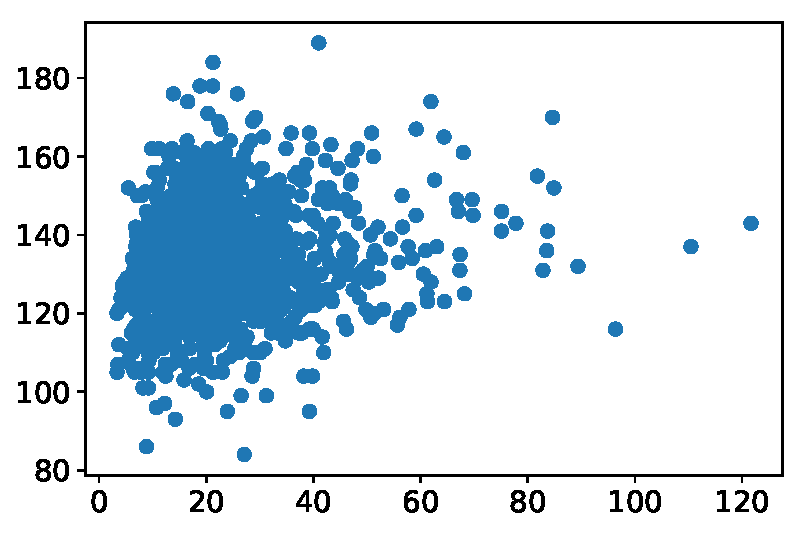
\includegraphics[scale=0.475]{data/Huang_et_al/huang_pm25vcirc_notitle.pdf}\vspace{10mm}\hspace{8mm}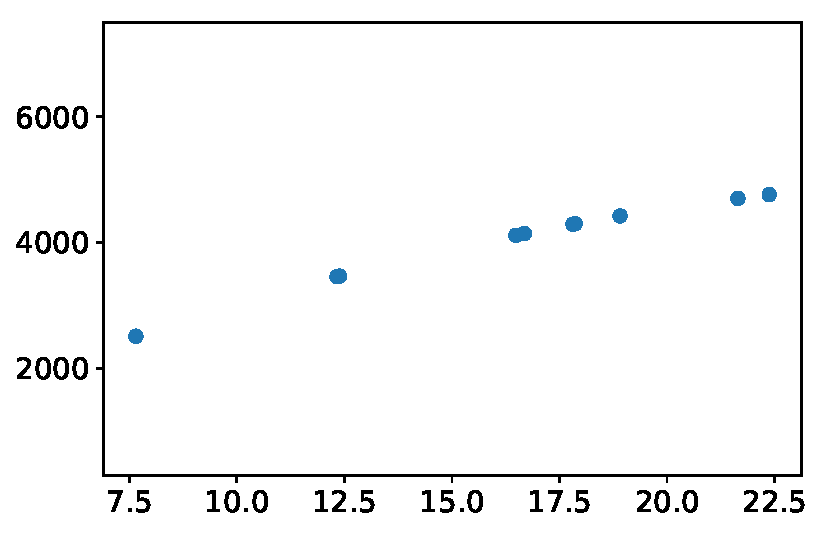
\includegraphics[scale=0.475]{data/Huang_et_al/projectile_notitle.pdf}

\end{frame}

\begin{frame}{Which is which?}


One is ER visits as a function of PM2.5 concentrations.  One is height of a rock as a function of time.

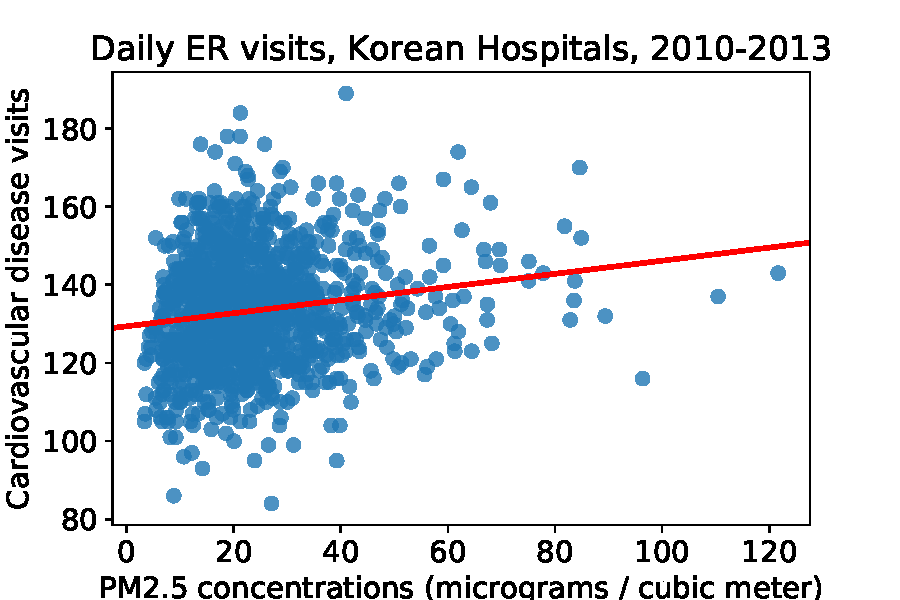
\includegraphics[scale=0.475]{data/Huang_et_al/huang_pm25vcirc_regplot.pdf}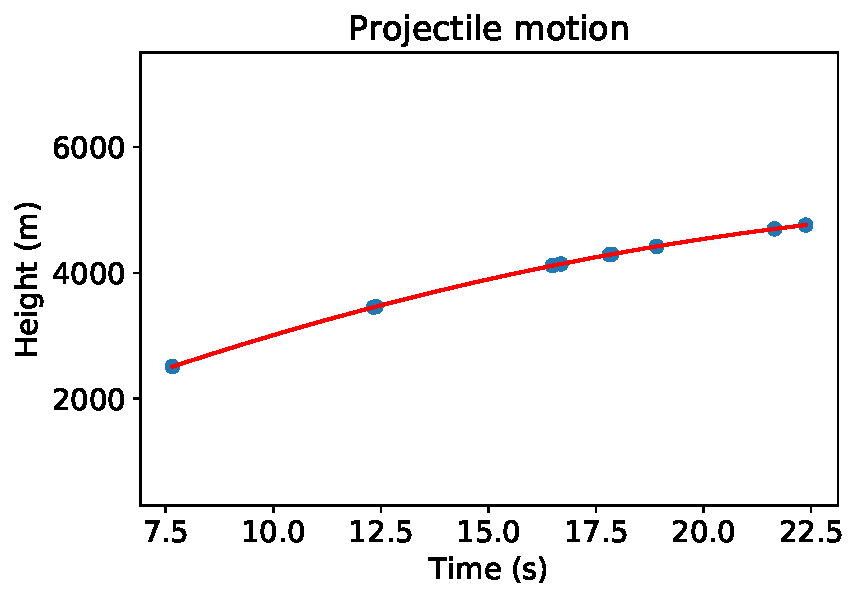
\includegraphics[scale=0.475]{data/Huang_et_al/projectile.pdf}

\begin{tiny}
Source for hospital data: Hwang, S. H. \textit{et al} (2017), PloS one, 12(8).
\end{tiny}

\end{frame}

\begin{frame}{How did you choose?}

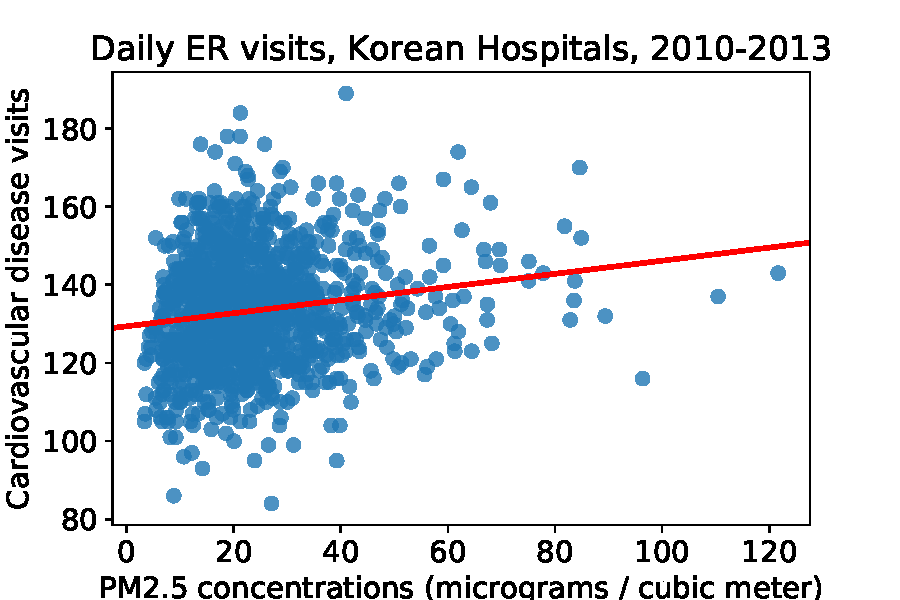
\includegraphics[scale=0.475]{data/Huang_et_al/huang_pm25vcirc_regplot.pdf}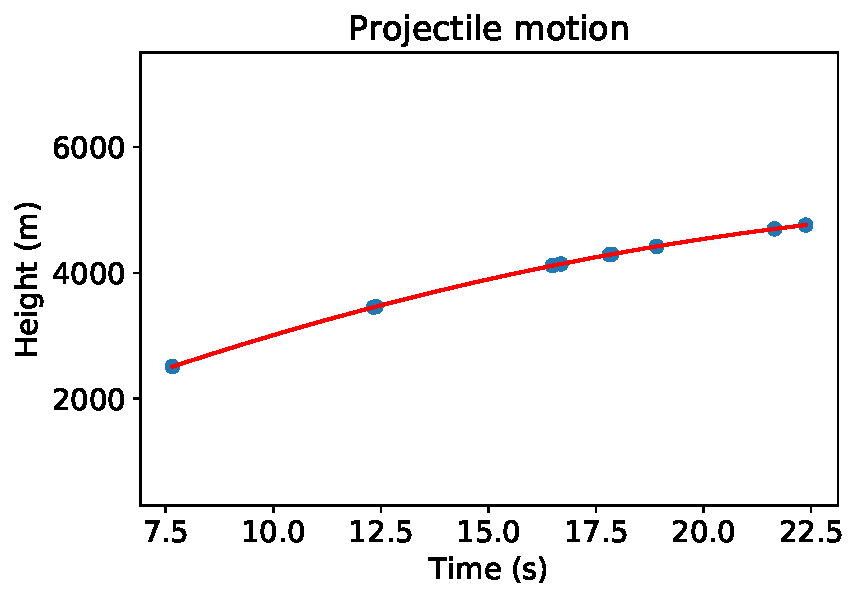
\includegraphics[scale=0.475]{data/Huang_et_al/projectile.pdf}

\begin{tiny}
Source for hospital data: Hwang, S. H. \textit{et al} (2017), PloS one, 12(8).
\end{tiny}

\pause

\begin{itemize}
\item The right plot has much less scatter
\item The right plot seems to be describing a more systematic process
\end{itemize}


\end{frame}


\begin{frame}{Could the projectile plot ever look like this?  How?}

\begin{columns}

\column{0.5\textwidth}
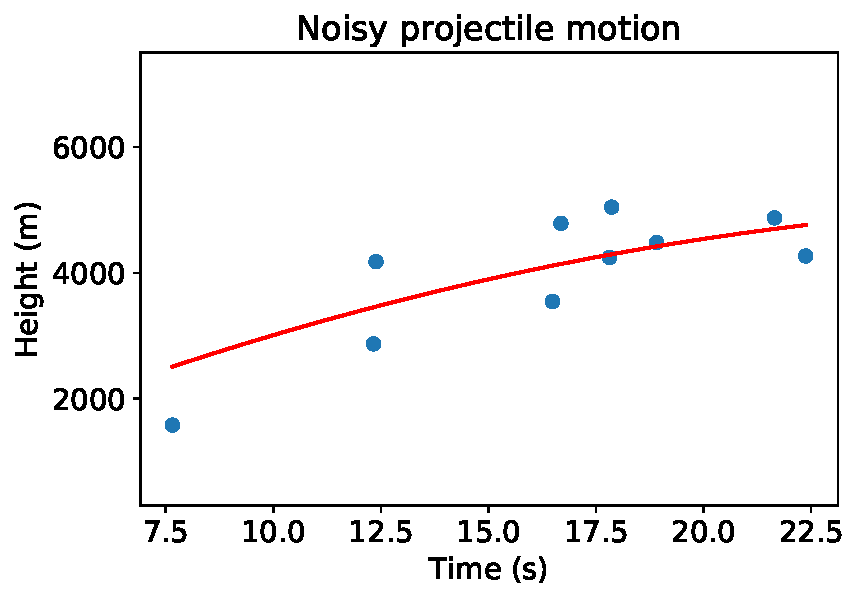
\includegraphics[scale=0.5]{data/Huang_et_al/projectile_noise.pdf}

\column{0.5\textwidth}

\pause

\begin{itemize}
\item Where could this noise come from?
\begin{itemize}
\item Measurement error
\item ``process noise,'' for example a windy environment.
\end{itemize}
\end{itemize}
\end{columns}

\end{frame}


\begin{frame}{Why might we build a model?}

\pause

Prediction.
\begin{itemize}
\item Where will the projectile be in 5 seconds?
\item I'm building a hospital in a city where I know the air quality trends as well as a bunch of other variables.  How big should the ER be?
\end{itemize}

\hspace{5mm}

Inference: Estimating a parameter
\begin{itemize}
\item What is the acceleration of gravity?
\item What is the correlation between air quality and ER visits?
\end{itemize}

\hspace{5mm}

\textit{Causal }Inference:
\begin{itemize}
\item Does PM2.5 cause heart attacks? 
\end{itemize} 

\end{frame}

\begin{frame}{Expectations for the model and data...}

Prediction:
\begin{itemize}
\item Low expectations! As long as the independent variables are correlated with the dependent variables, we can make predictions.
\end{itemize}
\hspace{2mm}

Inference: 
\begin{itemize}
\item Moderate expectations on the model: It needs to be sufficiently interpretable that we can understand what parameters mean
\end{itemize}
\hspace{2mm}

\textit{Causal }Inference:
\begin{itemize}
\item Very high expectations!  We need to be confident that \textit{only} the independent variable is changing systematically across measurements.  
\item Otherwise we can't rule out the possibility that some other unobserved variable is impacting our observations.
\end{itemize}

\end{frame}


\begin{frame}{You say regressor, I say feature}

\begin{table}[]
\begin{tabular}{lp{5.5cm}p{5.5cm}}
 \textbf{Math} & \textbf{Machine learning} & \textbf{Statistics}  \\
 \hline
 \hline
  $x$& \textbf{independent variable}, predictor, input variable, feature & \textbf{independent variable}, regressor, covariate,  explanatory variable, right hand variable \\
 $y$ &  \textbf{dependent variable}, output variable response variable & \textbf{dependent variable,} outcome variable, left-hand side variable.
\end{tabular}
\end{table}

\end{frame}


\begin{frame}{A little notation}
Moving forward, we'll use this notation and terminology:

\begin{eqnarray*}
x_i & i^\text{th} \text{ observation of an independent variable}\\
y_i & i^\text{th} \text{ observation of a dependent variable}\\
\epsilon_i & i^\text{th} \text{ random error, uncorrelated with }x_i,\text{ and mean zero}\\\\
y_i = f(x_i) + \epsilon_i & \text{ the ``true'' model, if one exists. }\\\\
\hat{y}_i = \hat{f}(x_i)  & \text{ our estimate of }y_i\text{ using an estimate of }f\\\end{eqnarray*}
\end{frame}

\begin{frame}{Error or residual?}

\begin{eqnarray*}
y_i = f(x_i) + \epsilon_i & \text{ the ``true'' model, if one exists. }\\
y_i = \hat{f}(x_i) + e_i & \text{ the relationship between the data and the estimate. }
\end{eqnarray*}

\hspace{5mm}
\pause

So:
\begin{eqnarray*}
\epsilon_i&\text{variation in $y$ that is uncorrelated with $x$.}\\
e_i = y_i - \hat{f}(x_i) & \text{ the ``residual'' between the data and the estimate. }
\end{eqnarray*}

\end{frame}

\begin{frame}{Error v. Residual, continued}

Important!  
\begin{itemize}
\item $\epsilon$ and $e$ could be very different.  
\item Because we'll rarely know the ``true'' model, we'll rarely know $\epsilon$.
\item On average, $e$ will never be smaller than $\epsilon$
\end{itemize}
\end{frame}

\begin{frame}{How to evaluate how well a model performs?}

Generic term: the \textit{Cost function.}

\begin{itemize}
\item Cost functions can be used to describe how much of the variation in the data can be captured by the model.
\item Example: The mean squared error:

\begin{align*}
MSE &= \frac{1}{n} ((y_1 - \hat{y}_1)^2 + (y_2 - \hat{y}_2)^2 + \cdots + (y_n - \hat{y}_n)^2) \\\\
&= \frac{1}{n} (e_1^2 + e_2^2 + \cdots + e_n^2) \\
&=\frac{1}{n} \sum_{i=1}^n e_i^2
\end{align*}
\end{itemize}

\end{frame}


\begin{frame}{A thought experiment from ISLR Ch 2}

\begin{columns}
\column{0.5\textwidth}
Suppose you have four different model forms to choose from.  When you fit them to the data, you get this figure.

\vspace{5mm}

Which model should you choose?  
\begin{itemize}
\item<2-> The one that minimizes mean squared error?
\item<3-> Careful!  Doesn't the squiggly one minimize mean squared error?
\item<4-> To do model selection we need to understand the concept of training and testing data.
\end{itemize}

\column{0.5\textwidth}
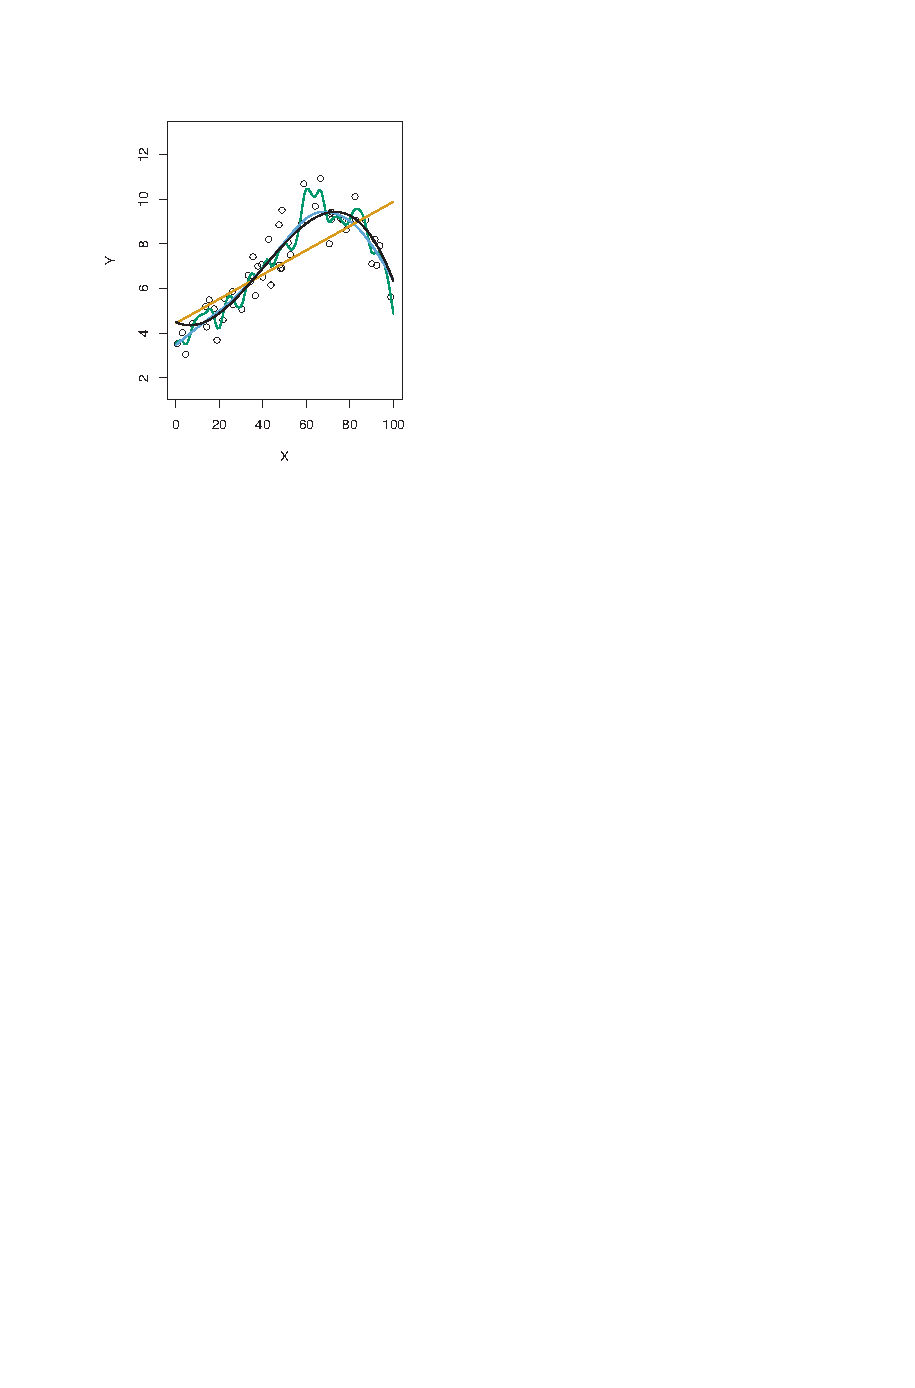
\includegraphics[scale=1]{figures/islr2_9a.pdf}
\end{columns}

\end{frame}

\begin{frame}{Concept:  Test and training data}


\begin{columns}
\column{0.65\textwidth}


Choosing between different models can be done by partitioning your data in to ``training'' and ``test'' data.

\begin{itemize}
\item ``Training data'': The data we use to choose the parameters of an individual model. 

\hspace{5mm}

\item ``Test data'': A set of data we withhold; it's not for training.  We use this data set to compare how different \textit{models} perform relative to one another.  

\end{itemize}
\column{0.35\textwidth}

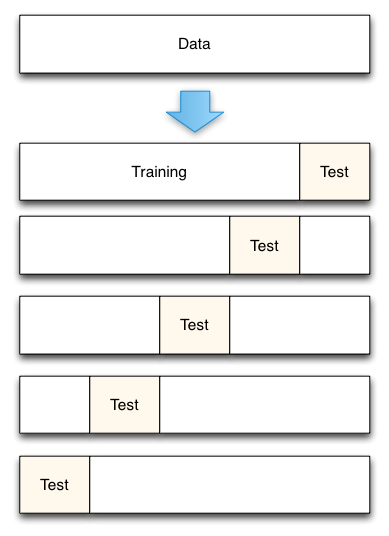
\includegraphics[scale=0.35]{figures/07_cross_validation_diagram}
\begin{tiny}
Source: kaggle.com
\end{tiny}
\end{columns}


\end{frame}


\begin{frame}{MSE for test and training data}


\begin{columns}
\column{0.5\textwidth}


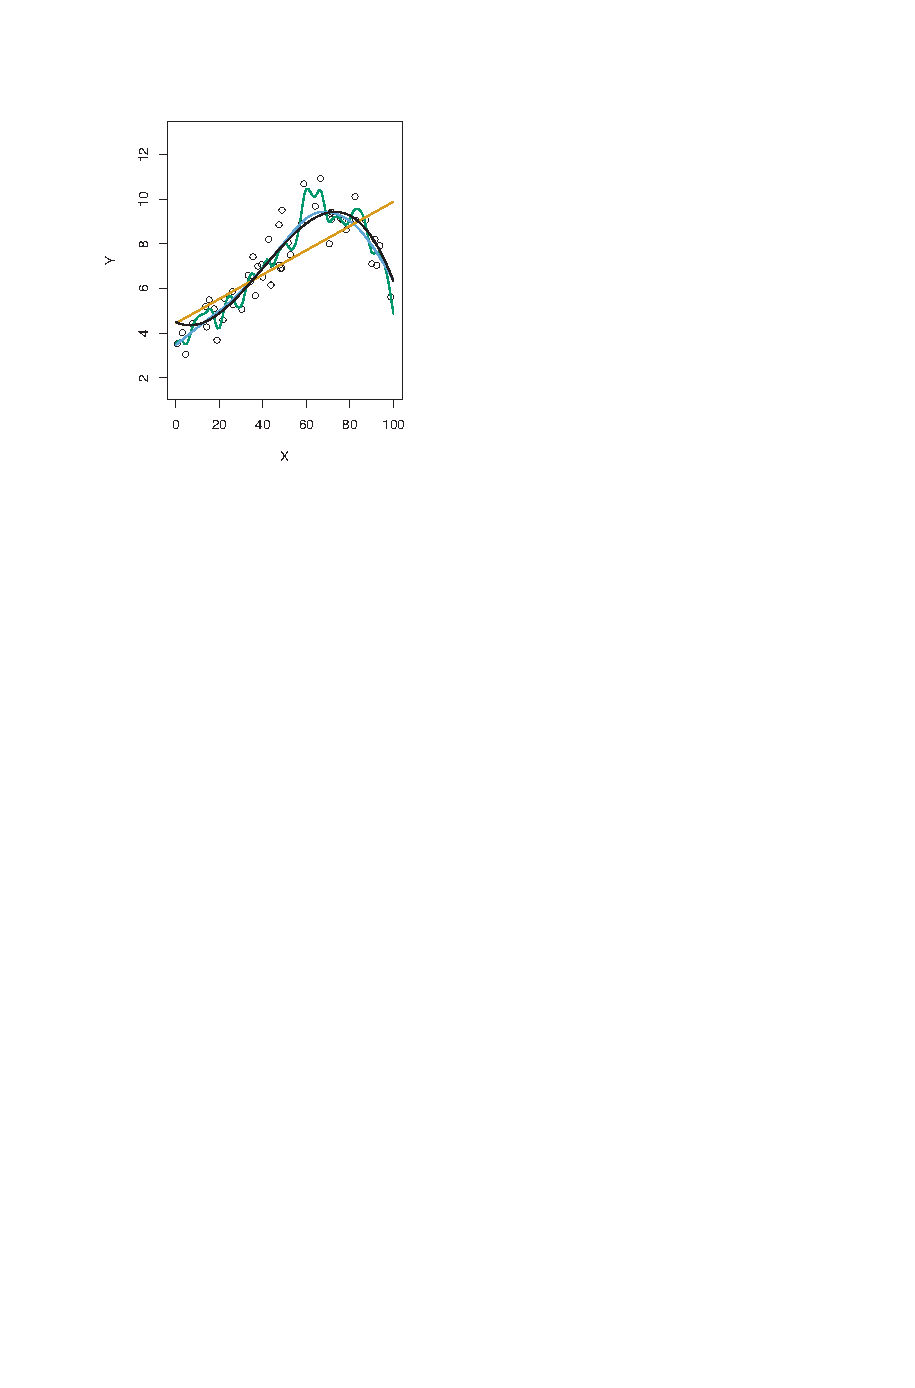
\includegraphics[scale=1]{figures/islr2_9a.pdf}


What might a plot of MSE versus model ``flexibility'' look like?


\column{0.5\textwidth}

\pause 
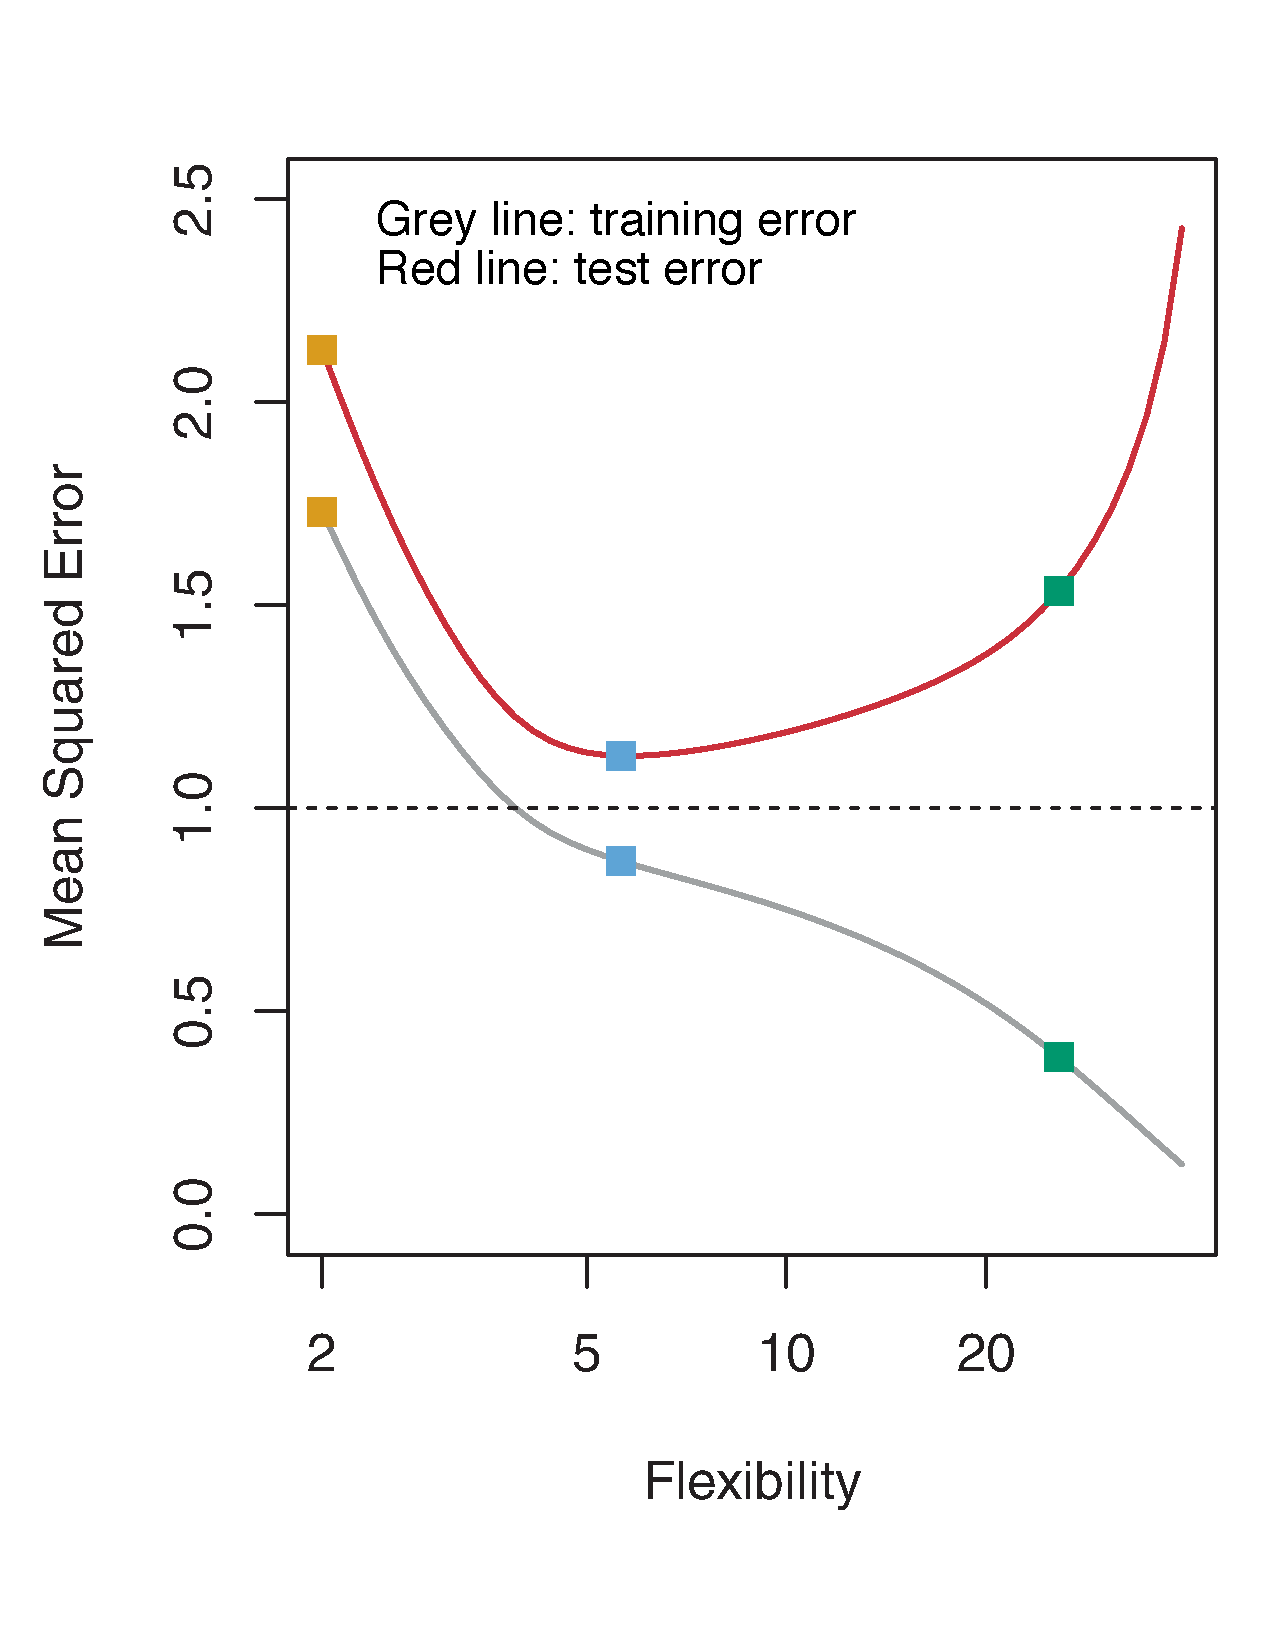
\includegraphics[scale=0.25]{figures/islr2_9b.pdf}
\end{columns}


\end{frame}


\begin{frame}{Bias v. Variance}

\textbf{Bias}: 
\begin{itemize}
\item The propensity for a model to produce errors that are systematically high or low
\item Bias can be positive in one range of the predictor and negative in another.  
\end{itemize}


\textbf{Variance}
\begin{itemize}
\item The propensity for a model to make very different predictions if it is fit with two different training data sets from the same process.
\end{itemize}

\hspace{5mm}

Total error can be decomposed:

\begin{align*}
\text{Average }(y_0-\hat{f}(x_0))^2 &=  \text{var} (\hat{f}(x_0)) + [\text{bias}(\hat{f}(x_0))]^2+\text{var}(\epsilon_0)
\end{align*}

\end{frame}


\begin{frame}{Bias v. Variance, ctd.}


\begin{columns}
\column{0.4\textwidth}

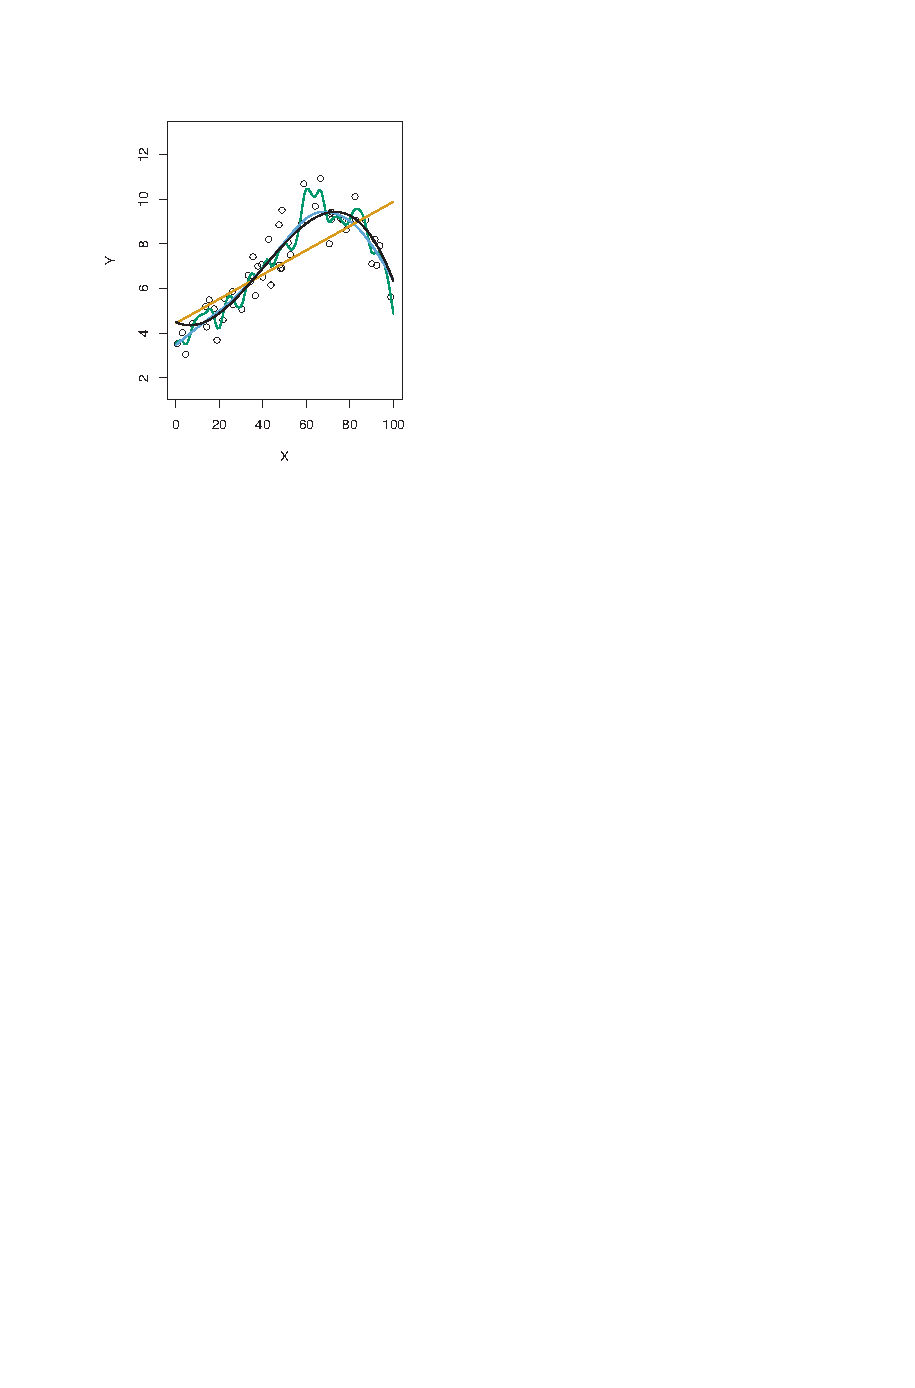
\includegraphics[scale=1]{figures/islr2_9a.pdf}

\column{0.6\textwidth}

Which model has the greatest propensity for bias?
\begin{itemize}
\item<2-> The linear one.  In ranges of $x$, it systematically under- or over-estimates. 
\end{itemize}

\hspace{5mm}

Which model has the greatest propensity for variance?
\begin{itemize}
\item<3-> The squiggly one.  If we drew another sample of data, we'd probably get very different squiggles.
\end{itemize}
\end{columns}



\end{frame}

\begin{frame}{Decomposing bias-variance}

\begin{columns}
\column{0.375\textwidth}
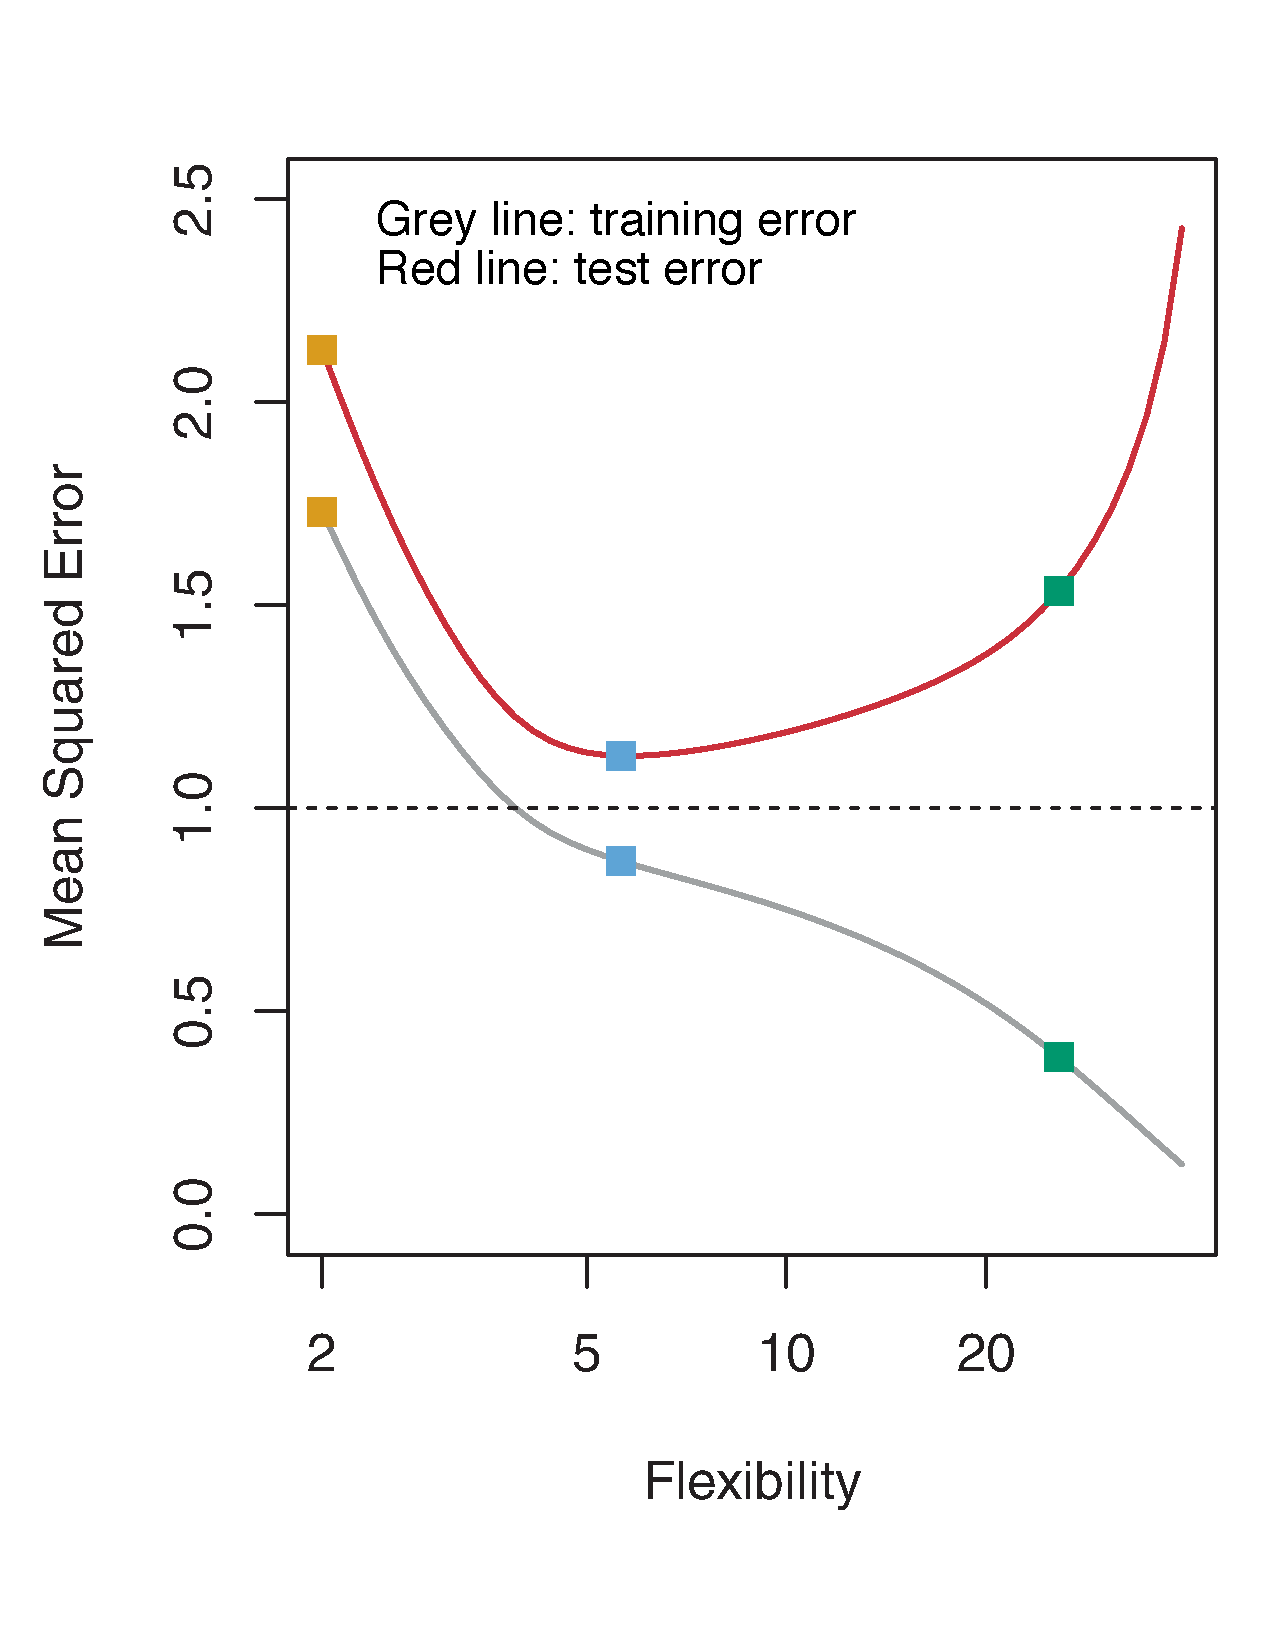
\includegraphics[scale=0.25]{figures/islr2_9b.pdf}

\column{0.3\textwidth}
Take a moment to think about how bias and variance add up to make the red curve on the left.  Try to draw bias and variance separately.  

\column{0.3\textwidth}
\pause 
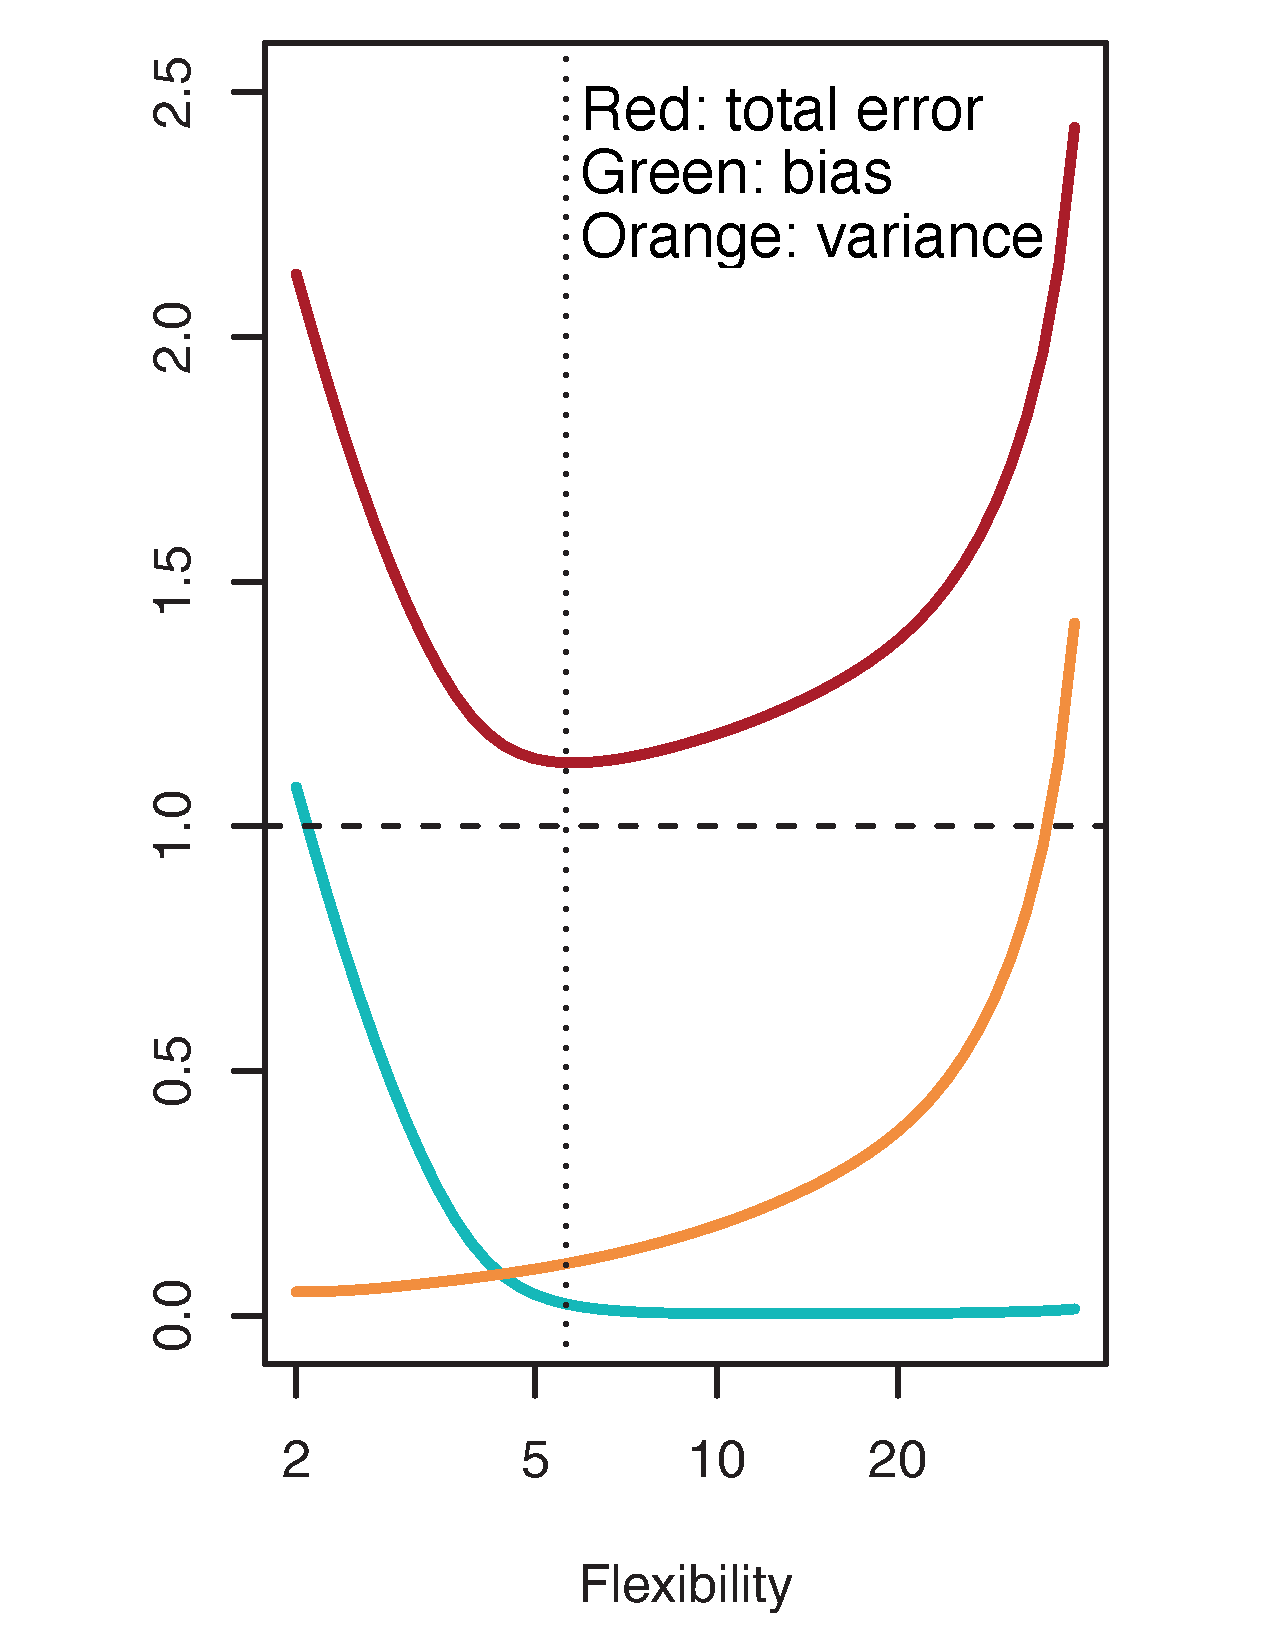
\includegraphics[scale=0.21]{figures/islr2_12a_text.pdf}

\end{columns}

\end{frame}
\end{document}


